% Options for packages loaded elsewhere
\PassOptionsToPackage{unicode}{hyperref}
\PassOptionsToPackage{hyphens}{url}
%
\documentclass[
]{article}
\usepackage{amsmath,amssymb}
\usepackage{lmodern}
\usepackage{iftex}
\ifPDFTeX
  \usepackage[T1]{fontenc}
  \usepackage[utf8]{inputenc}
  \usepackage{textcomp} % provide euro and other symbols
\else % if luatex or xetex
  \usepackage{unicode-math}
  \defaultfontfeatures{Scale=MatchLowercase}
  \defaultfontfeatures[\rmfamily]{Ligatures=TeX,Scale=1}
\fi
% Use upquote if available, for straight quotes in verbatim environments
\IfFileExists{upquote.sty}{\usepackage{upquote}}{}
\IfFileExists{microtype.sty}{% use microtype if available
  \usepackage[]{microtype}
  \UseMicrotypeSet[protrusion]{basicmath} % disable protrusion for tt fonts
}{}
\makeatletter
\@ifundefined{KOMAClassName}{% if non-KOMA class
  \IfFileExists{parskip.sty}{%
    \usepackage{parskip}
  }{% else
    \setlength{\parindent}{0pt}
    \setlength{\parskip}{6pt plus 2pt minus 1pt}}
}{% if KOMA class
  \KOMAoptions{parskip=half}}
\makeatother
\usepackage{xcolor}
\usepackage[margin=1in]{geometry}
\usepackage{color}
\usepackage{fancyvrb}
\newcommand{\VerbBar}{|}
\newcommand{\VERB}{\Verb[commandchars=\\\{\}]}
\DefineVerbatimEnvironment{Highlighting}{Verbatim}{commandchars=\\\{\}}
% Add ',fontsize=\small' for more characters per line
\usepackage{framed}
\definecolor{shadecolor}{RGB}{248,248,248}
\newenvironment{Shaded}{\begin{snugshade}}{\end{snugshade}}
\newcommand{\AlertTok}[1]{\textcolor[rgb]{0.94,0.16,0.16}{#1}}
\newcommand{\AnnotationTok}[1]{\textcolor[rgb]{0.56,0.35,0.01}{\textbf{\textit{#1}}}}
\newcommand{\AttributeTok}[1]{\textcolor[rgb]{0.77,0.63,0.00}{#1}}
\newcommand{\BaseNTok}[1]{\textcolor[rgb]{0.00,0.00,0.81}{#1}}
\newcommand{\BuiltInTok}[1]{#1}
\newcommand{\CharTok}[1]{\textcolor[rgb]{0.31,0.60,0.02}{#1}}
\newcommand{\CommentTok}[1]{\textcolor[rgb]{0.56,0.35,0.01}{\textit{#1}}}
\newcommand{\CommentVarTok}[1]{\textcolor[rgb]{0.56,0.35,0.01}{\textbf{\textit{#1}}}}
\newcommand{\ConstantTok}[1]{\textcolor[rgb]{0.00,0.00,0.00}{#1}}
\newcommand{\ControlFlowTok}[1]{\textcolor[rgb]{0.13,0.29,0.53}{\textbf{#1}}}
\newcommand{\DataTypeTok}[1]{\textcolor[rgb]{0.13,0.29,0.53}{#1}}
\newcommand{\DecValTok}[1]{\textcolor[rgb]{0.00,0.00,0.81}{#1}}
\newcommand{\DocumentationTok}[1]{\textcolor[rgb]{0.56,0.35,0.01}{\textbf{\textit{#1}}}}
\newcommand{\ErrorTok}[1]{\textcolor[rgb]{0.64,0.00,0.00}{\textbf{#1}}}
\newcommand{\ExtensionTok}[1]{#1}
\newcommand{\FloatTok}[1]{\textcolor[rgb]{0.00,0.00,0.81}{#1}}
\newcommand{\FunctionTok}[1]{\textcolor[rgb]{0.00,0.00,0.00}{#1}}
\newcommand{\ImportTok}[1]{#1}
\newcommand{\InformationTok}[1]{\textcolor[rgb]{0.56,0.35,0.01}{\textbf{\textit{#1}}}}
\newcommand{\KeywordTok}[1]{\textcolor[rgb]{0.13,0.29,0.53}{\textbf{#1}}}
\newcommand{\NormalTok}[1]{#1}
\newcommand{\OperatorTok}[1]{\textcolor[rgb]{0.81,0.36,0.00}{\textbf{#1}}}
\newcommand{\OtherTok}[1]{\textcolor[rgb]{0.56,0.35,0.01}{#1}}
\newcommand{\PreprocessorTok}[1]{\textcolor[rgb]{0.56,0.35,0.01}{\textit{#1}}}
\newcommand{\RegionMarkerTok}[1]{#1}
\newcommand{\SpecialCharTok}[1]{\textcolor[rgb]{0.00,0.00,0.00}{#1}}
\newcommand{\SpecialStringTok}[1]{\textcolor[rgb]{0.31,0.60,0.02}{#1}}
\newcommand{\StringTok}[1]{\textcolor[rgb]{0.31,0.60,0.02}{#1}}
\newcommand{\VariableTok}[1]{\textcolor[rgb]{0.00,0.00,0.00}{#1}}
\newcommand{\VerbatimStringTok}[1]{\textcolor[rgb]{0.31,0.60,0.02}{#1}}
\newcommand{\WarningTok}[1]{\textcolor[rgb]{0.56,0.35,0.01}{\textbf{\textit{#1}}}}
\usepackage{graphicx}
\makeatletter
\def\maxwidth{\ifdim\Gin@nat@width>\linewidth\linewidth\else\Gin@nat@width\fi}
\def\maxheight{\ifdim\Gin@nat@height>\textheight\textheight\else\Gin@nat@height\fi}
\makeatother
% Scale images if necessary, so that they will not overflow the page
% margins by default, and it is still possible to overwrite the defaults
% using explicit options in \includegraphics[width, height, ...]{}
\setkeys{Gin}{width=\maxwidth,height=\maxheight,keepaspectratio}
% Set default figure placement to htbp
\makeatletter
\def\fps@figure{htbp}
\makeatother
\setlength{\emergencystretch}{3em} % prevent overfull lines
\providecommand{\tightlist}{%
  \setlength{\itemsep}{0pt}\setlength{\parskip}{0pt}}
\setcounter{secnumdepth}{-\maxdimen} % remove section numbering
\renewcommand{\and}{\\}
\ifLuaTeX
  \usepackage{selnolig}  % disable illegal ligatures
\fi
\IfFileExists{bookmark.sty}{\usepackage{bookmark}}{\usepackage{hyperref}}
\IfFileExists{xurl.sty}{\usepackage{xurl}}{} % add URL line breaks if available
\urlstyle{same} % disable monospaced font for URLs
\hypersetup{
  pdftitle={Proyecto final: Análisis de alergias de usuarios de un recetario web},
  pdfauthor={INSTITUTO POLITÉCNICO NACIONAL; -----------------------------------------------------------; Alumno: Hector Isaac Roman Vazquez ------------ Boleta: 2021670099; Alumno: Jesús Eduardo Guijarro Saldaña -------- Boleta: 2021670220; Alumno: Omar Montoya Romero ------------------- Boleta: 2021670251; Alumno: Arnold Torres Maldonado ---------------- Boleta: 2021670117; -----------------------------------------------------------; Docente: Hector Alejandro Acuña Cid},
  hidelinks,
  pdfcreator={LaTeX via pandoc}}

\title{Proyecto final: Análisis de alergias de usuarios de un recetario
web}
\author{INSTITUTO POLITÉCNICO
NACIONAL \and ----------------------------------------------------------- \and Alumno:
Hector Isaac Roman Vazquez ------------ Boleta: 2021670099 \and Alumno:
Jesús Eduardo Guijarro Saldaña -------- Boleta: 2021670220 \and Alumno:
Omar Montoya Romero ------------------- Boleta: 2021670251 \and Alumno:
Arnold Torres Maldonado ---------------- Boleta:
2021670117 \and ----------------------------------------------------------- \and Docente:
Hector Alejandro Acuña Cid}
\date{16 de Junio del 2023}

\begin{document}
\maketitle

\hypertarget{abstract}{%
\section{Abstract}\label{abstract}}

This report reflects the data analysis process of a web system developed
by the authors of the document with the objective of identifying which
is the allergy that is most repeated, as well as the number of most
common allergies, in the same way makes use of the linear regression
tools and the KNN algorithm to make a comparison between the results
obtained from both methods and this, conclude that X is the most
accurate tool, the most repeated allergy is to pickles and the number of
most common allergies It's zero allergies.

\hypertarget{resumen}{%
\section{Resumen}\label{resumen}}

En este reporte se plasma el proceso de análisis de los datos de un
sistema web desarrollado por los autores del documento, Con los
objetivos de identificar cual es la alergia que mas se logra repetir,
asi como el número de alergias más común, de igual manera se hace uso de
las herramientas de regresión lineal y el algoritmo KNN para realizar
una comparacion entre los resultados obtenidos de ambos metodos y asi,
concluir que X es la herramienta más precisa, la alergia más repetida es
a los pepinillos y el número de alergias más común es cero alergias.

\hypertarget{introducciuxf3n}{%
\section{Introducción}\label{introducciuxf3n}}

En la siguiente investigación se utiliza una base de datos de
aproximadamente 600 usuarios de los cuales se pueden recuperar los datos
de los ingredientes a los que son alérgicos e incluso si alguno de los
usuarios no cuenta con alergias, para de esta manera poder realizar una
análisis utilizando regresión lineal y el algoritmo KNN, para poder
hacer una comparativa entre ambos, mediante la metodología CRISP-DM para
lograr un mejor análisis.

\hypertarget{marco-teuxf3rico}{%
\section{Marco teórico}\label{marco-teuxf3rico}}

Una alergia es una reacción de su sistema inmunitario hacia algo que no
molesta a la mayoría de las demás personas. Quienes tienen alergias
suelen ser sensibles a más de una cosa. Las sustancias que suelen causar
reacciones son: {[}4{]}

\begin{itemize}
\item
  Polen
\item
  Ácaros del polvo
\item
  Esporas de moho
\item
  Caspa de animales
\item
  Alimentos
\item
  Picaduras de insectos
\item
  Medicinas
\end{itemize}

Las alergias pueden provocar una serie de síntomas como goteos nasales,
estornudos, picazón, sarpullidos, edema (hinchazón) o asma. Las alergias
van de leves a severas. Una reacción severa llamada anafilaxia puede
resultar fatal. Los médicos usan pruebas de piel y sangre para
diagnosticar las alergias. Los tratamientos incluyen medicinas,
inyecciones y evitar las sustancias que causan las alergias. {[}4{]}

Una alergia alimentaria es una reacción del sistema inmunitario que
ocurre poco después de haber ingerido un determinado alimento. Incluso
una pequeña cantidad del alimento que causa la alergia puede ocasionar
signos y síntomas, como problemas digestivos, urticaria o inflamación de
las vías respiratorias. En algunos casos, una alergia alimentaria puede
ocasionar síntomas graves o, incluso, una reacción que puede poner en
riesgo la vida, llamada anafilaxia. {[}5{]}

\begin{figure}
\centering

\includegraphics[width=0.3\textwidth,height=\textheight]{D:/Escritorio/IPN Upiiz/6ª Semestre/Mineria de datos/reporte/ALERGI.jpg}
\caption{Aleriga alimentaria.}
\end{figure}

Se calcula que la alergia alimentaria afecta al 8 por ciento de los
niños menores de 5 años y hasta al 4 por ciento de los adultos. A pesar
de que no existe cura, algunos niños superan sus alergias alimentarias
cuando crecen. {[}5{]}

La alergia alimentaria puede fácilmente confundirse con una reacción
mucho más frecuente llamada intolerancia alimentaria. Si bien es
molesta, la intolerancia alimentaria es una afección de menor gravedad
que no involucra al sistema inmunitario si no que, significa que el
cuerpo de la persona no puede digerir bien determinado alimento, o que
un alimento en particular le irrita el sistema digestivo. Entre los
síntomas de la intolerancia alimentaria, se incluyen los siguientes:
náuseas, gases, retortijones, dolor abdominal, diarrea, irritabilidad y
dolor de cabeza. {[}2{]}

los ``Datasets'', son fundamentales para la revolución del procesamiento
de datos por la que estamos pasando, y muchas veces, más sencillos de lo
que parecen. Un Dataset no es más que un conjunto de datos tabulados en
cualquier sistema de almacenamiento de datos estructurados. El término
Dataset hace referencia a una única base de datos de origen, la cual se
puede relacionar con otras, cada columna del Dataset representa una
variable y cada fila corresponde a cualquier dato que estemos tratando.
{[}1{]}

Existen cuatro tipos de Datasets catalogados según su origen y formato,
los cuales son usados según las necesidades de los modelos de datos a
trabajar. {[}1{]}

\begin{itemize}
\tightlist
\item
  Archivo: es un fichero independiente en el que se almacena toda la
  información con la que se va a trabajar del Dataset. Tiene como
  ventajas, la seguridad y rapidez para el trabajo con los datos, ya que
  siempre se explotan y se visualizan de manera local, sin embargo la
  escalabilidad y conexión con otros Datasets que no están almacenados
  en la misma máquina se dificulta.
\end{itemize}

\begin{itemize}
\tightlist
\item
  Folder: es la suma de diferentes Datasets almacenados en una misma
  carpeta, los cuales están conectados entre ellos. Estos archivos deben
  compartir un mismo formato como puede ser .csv, .mif o dxf.
\end{itemize}

\begin{itemize}
\tightlist
\item
  de datos: este tipo de Dataset puede llegarse a confundir con el
  archivo, pero se diferencia por su nivel de especialidad, es decir,
  son bases de datos con formatos específicos diseñadas para programas
  puntuales. Por ejemplo las bases de datos de Oracle, las cuales solo
  funcionan para sus desarrollos.
\end{itemize}

\begin{itemize}
\tightlist
\item
  Web: es la compilación de datos que se almacenan dentro de un sitio
  web del Dataset. El nombre que se le asigna por defecto a este Dataset
  es el correspondiente a la URL.
\end{itemize}

\hypertarget{materiales-y-muxe9todos}{%
\section{Materiales y métodos}\label{materiales-y-muxe9todos}}

\hypertarget{r-y-rstudio}{%
\subsection{R y RStudio}\label{r-y-rstudio}}

Para la investigación se usó el lenguaje de programación R, R es un
lenguaje de programación estadística ampliamente utilizado para análisis
de datos, modelado estadístico y visualización. Es una plataforma
gratuita y de código abierto que ofrece una amplia gama de herramientas
y paquetes especializados para el procesamiento y análisis de datos.
RStudio, por otro lado, es un entorno de desarrollo integrado (IDE)
diseñado específicamente para trabajar con R. Proporciona una interfaz
gráfica fácil de usar que facilita la escritura, ejecución y depuración
de código en R. RStudio también ofrece características adicionales como
paneles de visualización, administración de proyectos y colaboración en
línea, lo que lo convierte en una herramienta popular entre los usuarios
de R {[}8{]}.

\hypertarget{modelo-crisp-dm}{%
\subsection{Modelo CRISP-DM}\label{modelo-crisp-dm}}

Para desarrollar los modelos y análisis correspondiente hicimos uso de
la metodología Cross Industry Standard Process for Data Mining (CRISP-DM
por sus siglas), esta es una metodología para la minería de datos que se
utiliza comúnmente en el análisis de datos empresariales. La metodología
consta de seis fases {[}6{]}:

\textbf{\emph{Comprensión del negocio/problema}}

El objetivo de esta fase es alinear los objetivos del proyecto de data
mining con los objetivos del negocio. Tratando así de evitar embarcarnos
en un proyecto de minería de datos que no produzca ningún efecto real en
la organización.

En esta fase deberemos ser capaces de:

\begin{itemize}
\tightlist
\item
  Establecer los objetivos de negocio.
\item
  Evaluar la situación actual.
\item
  Fijar los objetivos a nivel de minería de datos.
\item
  Obtener un plan de proyecto.
\end{itemize}

\textbf{\emph{Comprensión de los datos}}

Dos puntos clave en esta fase: conocer los datos, estructura y
distribución, y la calidad de estos.

En esta fase deberemos ser capaces de:

\begin{itemize}
\tightlist
\item
  Ejecutar procesos de captura de datos.
\item
  Proporcionar una descripción del juego de datos.
\item
  Realizar tareas de exploración de datos.
\item
  Gestionar la calidad de los datos, identificando problemas y
  proporcionando - - soluciones.
\end{itemize}

\textbf{\emph{Preparación de los datos}}

El objetivo final de esta fase es obtener los datos finales sobre los
que aplicarán los modelos.

En esta fase deberemos ser capaces de:

\begin{itemize}
\tightlist
\item
  Establecer el universo de datos con los que trabajar.
\item
  Realizar tareas de limpieza de datos.
\item
  Construir un juego de datos apto para ser usado en modelos de minería
  de - - - datos.
\item
  Integrar datos de fuentes heterogéneas si es necesario.
\end{itemize}

\textbf{\emph{Modelado}}

El objetivo último de esta fase es construir un modelo que nos permita
alcanzar los objetivos del proyecto.

En esta fase deberemos ser capaces de:

\begin{itemize}
\tightlist
\item
  Seleccionar las técnicas de modelado más adecuadas para nuestro juego
  de datos y nuestros objetivos.
\item
  Fijar una estrategia de verificación de la calidad del modelo.
\item
  Construir un modelo a partir de la aplicación de las técnicas
  seleccionadas sobre el juego de datos.
\item
  Ajustar el modelo evaluando su fiabilidad y su impacto en los
  objetivos anteriormente establecidos.
\end{itemize}

\textbf{\emph{Evaluación del modelo}}

En esta fase se centra en evaluar el grado de acercamiento del modelo a
los objetivos.

En esta fase deberemos ser capaces de:

\begin{itemize}
\tightlist
\item
  Evaluar el modelo o modelos generados hasta el momento.
\item
  Revisar todo el proceso de minería de datos que se ha llevado hasta
  este punto.
\item
  Establecer los siguientes pasos a tomar, tanto si se trata de repetir
  fases anteriores como si se trata de abrir nuevas líneas de
  investigación.
\end{itemize}

\textbf{\emph{Implementación}}

El objetivo de esta fase es realizar la implementación de los resultados
obtenidos de forma que sea propagado a los usuarios finales así como el
mantenimiento de este una vez la implementación haya finalizado.

En esta fase deberemos ser capaces de:

\begin{itemize}
\tightlist
\item
  Diseñar un plan de despliegue de modelos y conocimiento sobre nuestra
  organización.
\item
  Realizar seguimiento y mantenimiento de la parte más operativa del
  despliegue.
\item
  Revisar el proyecto en su globalidad con el objetivo de identificar
  lecciones aprendidas. {[}9{]}
\end{itemize}

\hypertarget{la-regresiuxf3n-lineal}{%
\subsection{La regresión lineal}\label{la-regresiuxf3n-lineal}}

Por otra parte, la regresión lineal es una técnica conocida de modelado
estadístico que se utiliza para analizar la relación entre dos variables
continuas. Se utiliza para predecir el valor de una variable dependiente
a partir del valor de una o más variables independientes, esta asume que
la relación entre las variables es lineal, lo que significa que el
cambio en la variable independiente tiene un cambio proporcional en la
variable dependiente. Una forma de aplicar la regresión lineal es
mediante el método de mínimos cuadrados, este es un método matemático
utilizado para encontrar una línea de regresión que mejor se ajusta a
los datos {[}7{]}. El objetivo del método es minimizar la suma de los
cuadrados de las diferencias entre los valores observados y los valores
predichos por la línea de regresión.

\hypertarget{el-algoritmo-knn-k-vecinos-muxe1s-cercanos}{%
\subsection{El algoritmo KNN (K vecinos más
cercanos)}\label{el-algoritmo-knn-k-vecinos-muxe1s-cercanos}}

Es un algoritmo de clasificación supervisada que usa la proximidad (por
ejemplo la distancia euclidiana) para hacer clasificaciones y
predicciones sobre agrupaciones de datos partiendo del supuesto de que
se pueden encontrar puntos similares cerca el uno del otro. Para hacer
predicciones sobre clasificaciones se toma el promedio de los k vecinos
más cercanos, estas predicciones se pueden hacer para valores continuos
mientras que las clasificaciones se hacen solo para valores discretos.

\hypertarget{conjunto-de-datos-de-alergias}{%
\subsection{Conjunto de datos de
alergias}\label{conjunto-de-datos-de-alergias}}

El conjunto de datos que se analizó proviene de un sistema web de
recetas donde los usuarios se dan de alta y especifican los ingredientes
a los cuales son alérgicos, el sistema los guarda en una base de datos
es ahí de donde nosotros obtuvimos el conjunto para trabajar {[}9{]}.

Algunas de las ventajas de este algoritmo son que es fácil de
implementar dado que solo requiere de un valor de k que elige el
analista y una métrica de distancia. Otra es que representa un buen
material didáctico dada su simplicidad y precisión por lo dicho
anteriormente {[}9{]}.

\hypertarget{experimentaciuxf3n-y-resultados}{%
\section{Experimentación y
resultados}\label{experimentaciuxf3n-y-resultados}}

\hypertarget{comprensiuxf3n-del-problema}{%
\subsection{Comprensión del
problema}\label{comprensiuxf3n-del-problema}}

Se genera una comparacion entre los resultados que se pueden obtener de
el analisis de usuarios con distintas alergias por medio de regresion
lineal haciendo uso de la metodologia CRISP-DM, haci como el analisis
por medio de knn de igual manera utilizando el mismo metodo de CRISP-DM.

Dichos datos se obtienen utilizando un conjunto de datos obtenidos
mendiante un sistema web, el sistema consta de un recetario, donde una
vez que se ingresa a la plataforma, el usuario puede seleccionar si se
tienen alergias a algun alimento, dichos datos se almacenan en una base
de datos y de ahi es posible que nosotros los extraigamos en un dataset
para poder realizar el analisis.

\hypertarget{entendimiento-de-los-datos}{%
\subsection{Entendimiento de los
datos}\label{entendimiento-de-los-datos}}

Usamos un conjunto de datos con 7 variables las cuales eran:

\begin{itemize}
\tightlist
\item
  Names: los nombres de los usuarios registrados en el sistema.
\end{itemize}

\begin{itemize}
\tightlist
\item
  lastNames: los apellidos de dichos usuarios.
\end{itemize}

\begin{itemize}
\tightlist
\item
  email: correo electrónico de los usuarios.
\end{itemize}

\begin{itemize}
\tightlist
\item
  password: contraseña de los usuarios.
\end{itemize}

\begin{itemize}
\tightlist
\item
  alergias: ingredientes a los que cada usuario era alérgico.
\end{itemize}

\begin{itemize}
\tightlist
\item
  numero\_alergias: número de ingredientes a los que el usuario era
  alérgico.
\end{itemize}

\hypertarget{preparaciuxf3n-de-los-datos}{%
\subsection{Preparación de los
datos}\label{preparaciuxf3n-de-los-datos}}

El archivo CSV que contenía los datos tenía las columnas separadas por
punto y coma y los ingredientes estaban separados por comas de la
siguiente manera:

\begin{Shaded}
\begin{Highlighting}[]
\NormalTok{Names;lastNames;email;password;alergias;numero\_alergias}
\NormalTok{Valeria;Flores;valeriaflores117@example.com;Vwx234@\#$;Camarones, Aceitunas;2}
\end{Highlighting}
\end{Shaded}

Por lo tanto para hacer los análisis correspondientes importamos dicho
archivo especificando el caracter que separaba las columnas con la línea
de código siguiente:

\begin{Shaded}
\begin{Highlighting}[]
\NormalTok{data }\OtherTok{\textless{}{-}} \FunctionTok{read.csv}\NormalTok{(}\StringTok{"usuarios.csv"}\NormalTok{, }\AttributeTok{sep=}\StringTok{";"}\NormalTok{)}
\end{Highlighting}
\end{Shaded}

\hypertarget{modelado}{%
\subsection{Modelado}\label{modelado}}

\hypertarget{encontrando-la-alergia-muxe1s-frecuente}{%
\subsubsection{Encontrando la alergia más
frecuente}\label{encontrando-la-alergia-muxe1s-frecuente}}

Para encontrar la alergia más frecuente hicimos un vector que contenía
todos los ingredientes repetidos.

\begin{Shaded}
\begin{Highlighting}[]
\CommentTok{\# strsplit para dividir los nombres separados por coma}
\CommentTok{\# en elementos individuales}
\NormalTok{ingredientes\_separados }\OtherTok{\textless{}{-}} \FunctionTok{strsplit}\NormalTok{(data}\SpecialCharTok{$}\NormalTok{alergias, }\StringTok{","}\NormalTok{)}
\CommentTok{\# unlist para crear un vector para poner los nombres separados}
\NormalTok{ingredientes }\OtherTok{\textless{}{-}} \FunctionTok{unlist}\NormalTok{(ingredientes\_separados)}
\end{Highlighting}
\end{Shaded}

Para empezar realizamos una tabla de frecuencias para los ingredientes
que nos permitió observar cuáles se repetían más, después esta tabla se
ordenó de manera descendente según su frecuencia para después tomar el
valor en la posición número 1, por último se imprime el resultado.

\begin{Shaded}
\begin{Highlighting}[]
\CommentTok{\# Cargar el dataset}
\NormalTok{data }\OtherTok{\textless{}{-}} \FunctionTok{read.csv}\NormalTok{(}\StringTok{"usuarios.csv"}\NormalTok{, }\AttributeTok{sep=}\StringTok{";"}\NormalTok{)}

\CommentTok{\# Calcular la frecuencia de las alergias}
\CommentTok{\# strsplit para dividir los nombres separados por coma}
\CommentTok{\# en elementos individuales}
\NormalTok{ingredientes\_separados }\OtherTok{\textless{}{-}} \FunctionTok{strsplit}\NormalTok{(data}\SpecialCharTok{$}\NormalTok{alergias, }\StringTok{","}\NormalTok{)}

\CommentTok{\# unlist para crear un vector para poner los nombres separados}
\NormalTok{ingredientes }\OtherTok{\textless{}{-}} \FunctionTok{unlist}\NormalTok{(ingredientes\_separados)}
\NormalTok{tabla\_de\_frecuencia }\OtherTok{\textless{}{-}} \FunctionTok{table}\NormalTok{(ingredientes)}

\CommentTok{\# ordenar de mayor a menor las frecuencias}
\NormalTok{alergias\_ordenadas }\OtherTok{\textless{}{-}} \FunctionTok{sort}\NormalTok{(tabla\_de\_frecuencia, }\AttributeTok{decreasing =} \ConstantTok{TRUE}\NormalTok{)}
\NormalTok{alergia\_mas\_comun }\OtherTok{\textless{}{-}} \FunctionTok{names}\NormalTok{(alergias\_ordenadas)[}\DecValTok{1}\NormalTok{] }\CommentTok{\# alergia ubicada en el \#1}

\CommentTok{\# Mostrar el resultado}
\FunctionTok{cat}\NormalTok{(}\StringTok{"La alergia más común es:"}\NormalTok{, alergia\_mas\_comun)}
\end{Highlighting}
\end{Shaded}

\begin{verbatim}
## La alergia más común es: Pepinillos
\end{verbatim}

\hypertarget{encontrando-el-nuxfamero-de-alergias-muxe1s-frecuente}{%
\subsubsection{Encontrando el número de alergias más
frecuente}\label{encontrando-el-nuxfamero-de-alergias-muxe1s-frecuente}}

Para esta sección también se hizo uso de una tabla de frecuencias que
ordenamos de manera descendente según el número de veces que se repetía
una cantidad de alergias. De nueva cuenta se seleccionó el valor en la
posición número 1 para después imprimir el resultado.

\begin{Shaded}
\begin{Highlighting}[]
\CommentTok{\# Cargar el dataset}
\NormalTok{data }\OtherTok{\textless{}{-}} \FunctionTok{read.csv}\NormalTok{(}\StringTok{"usuarios.csv"}\NormalTok{, }\AttributeTok{sep=}\StringTok{";"}\NormalTok{)}
\CommentTok{\# elegir la columna numero\_alergias del DS}
\NormalTok{num\_alergias }\OtherTok{\textless{}{-}}\NormalTok{ data}\SpecialCharTok{$}\NormalTok{numero\_alergias}
\CommentTok{\# tabla de frecuencias de los numeros de alergias}
\NormalTok{frecuencia }\OtherTok{\textless{}{-}} \FunctionTok{table}\NormalTok{(num\_alergias)}
\CommentTok{\# ordenar frecuencias de la tabla de manera descendente}
\NormalTok{frecuencia\_num\_ordenadas }\OtherTok{\textless{}{-}} \FunctionTok{sort}\NormalTok{(frecuencia,}\AttributeTok{decreasing =} \ConstantTok{TRUE}\NormalTok{)}
\CommentTok{\# elegir la alergia \#1}
\NormalTok{num\_alergia\_mas\_frecuente }\OtherTok{\textless{}{-}} \FunctionTok{names}\NormalTok{(frecuencia\_num\_ordenadas)[}\DecValTok{1}\NormalTok{]}

\CommentTok{\# imprimir solución}
\FunctionTok{cat}\NormalTok{(}\StringTok{"Es más común que los usuarios tengan"}\NormalTok{, num\_alergia\_mas\_frecuente, }\StringTok{"alergias"}\NormalTok{)}
\end{Highlighting}
\end{Shaded}

\begin{verbatim}
## Es más común que los usuarios tengan 0 alergias
\end{verbatim}

\hypertarget{uso-del-algoritmo-knn}{%
\subsubsection{Uso del algoritmo KNN}\label{uso-del-algoritmo-knn}}

XXXXXXXXXXXXXXXXXXXXXXXXXXXXXXXXXXXXXX

\hypertarget{uso-de-la-tuxe9cnica-de-regresiuxf3n-lineal}{%
\subsubsection{Uso de la técnica de regresión
lineal}\label{uso-de-la-tuxe9cnica-de-regresiuxf3n-lineal}}

XXXXXXXXXXXXXXXXXXXXXXXXXXXXXXXXXXXXXX

\hypertarget{resultados-del-modelo}{%
\subsection{Resultados del modelo}\label{resultados-del-modelo}}

El análisis que se realizó a partir de tablas de frecuencia muestra que
el número de alergias más frecuente es el de cero con 221 usuarios,
seguido de tres, uno, cuatro, dos y cinco alergias.

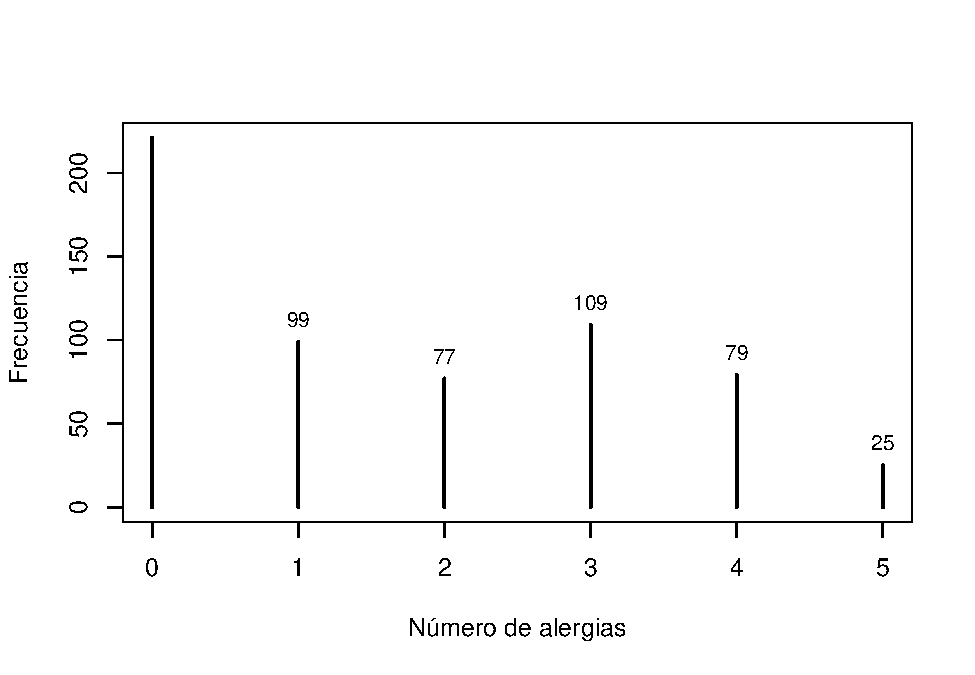
\includegraphics{reporte_files/figure-latex/unnamed-chunk-5-1.pdf}

También muestra que el ingrediente al cual los usuarios son más
alérgicos son los pepinillos seguido de las espinacas, el cilantro, el
tomate y la berenjena.

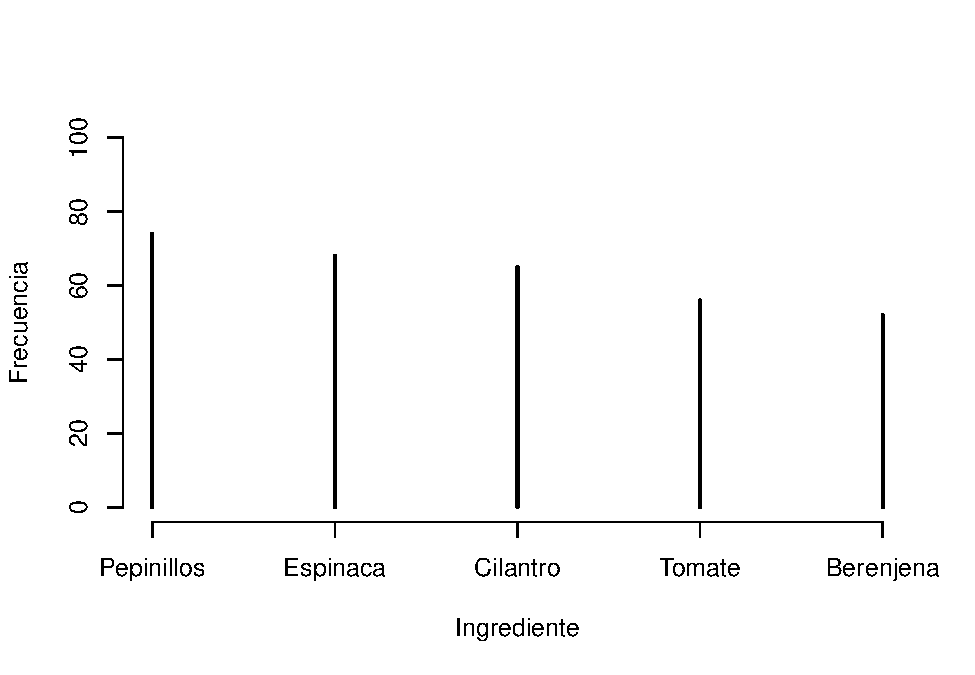
\includegraphics{reporte_files/figure-latex/unnamed-chunk-6-1.pdf}

\hypertarget{conclusiones}{%
\section{Conclusiones}\label{conclusiones}}

XXXXXXXXXXXXXXXXXXXXXXXXXXXXXXXXXXXXXX

\hypertarget{referencias}{%
\section{Referencias}\label{referencias}}

{[}1{]} ``¿Qué son los Datasets? {[}4 sitios donde encontrarlos{]}'',
KeepCoding Bootcamps, 27-feb-2020.

{[}2{]} ``¿En qué se diferencia una alergia alimentaria de una
intolerancia alimentaria?'', Kidshealth.org. {[}En línea{]}. Disponible
en: \url{https://kidshealth.org/es/parents/allergy-intolerance.html.}
{[}Consultado: 07-jun-2023{]}.

{[}3{]} ``Alergia'', Ear, Nose and Throat, 2002.

{[}4{]} ``Alergias'', Mayoclinic.org, 05-ago-2022. {[}En línea{]}.
Disponible en:
\url{https://www.mayoclinic.org/es-es/diseases-conditions/allergies/symptoms-causes/syc-20351497.}
{[}Consultado: 07-jun-2023{]}.

{[}5{]} A. A. Medina, S. M. Armentia, y S. F. Cortés, ``Alergia
alimentaria'', Medicine, vol.~13, núm. 28, pp.~1572--1578, 2021.

{[}6{]} IBM. (2021). Conceptos básicos de ayuda de CRISP-DM. {[}En
línea{]}. Disponible en:
\url{https://www.ibm.com/docs/es/spss-modeler/saas?topic=dm-crisp-help-overview}.
{[}Consultado: 07-jun-2023{]}.

{[}7{]} Online Statistics Education: A Multimedia Course of Study.
(2019). Linear Regression. Disponible en:
{[}\url{http://onlinestatbook.com/2/regression/intro.html}{]}.
{[}Consultado: 07-jun-2023{]}.

{[}8{]} Wickham, H., \& Grolemund, G. (2017). R for Data Science.
O'Reilly Media.

{[}9{]} IBM. (2021). ¿Qué es KNN?. {[}En línea{]}. Disponible en:
\url{https://www.ibm.com/mx-es/topics/knn} . {[}Consultado:
07-jun-2023{]}.

\end{document}
